\section{Introduction}
\label{sec:intro}

Offerings of massively open online courses (MOOCs) have been expanding
over the past years. Companies are betting their existence on the
continuation of this trend. Universities are experimenting to find
their own approaches, either to teaching open classes, or to develop
courses directed to their enrolled students. Thus, while the embrace
of the `massive,' and `open' portions of MOOCs might vary, the
`online' aspect as a tool for teaching is gaining ground, and we focus
on this aspect here. Best practices for the use of the Internet to
teach are still evolving, and not all voices are enthusiastic
\cite{Eckerdal2014}. Nonetheless, given the trend it is essential to
develop technologies that take maximum advantage of the online medium.

Current course offerings expose many opportunities for such
technologies. Peer assessment, forum use, guided tutoring, and
interventions that address dropout rates all offer such possibilities
for technological improvement \cite{Piech2013,
  balfour2013,Coetzee2014, agrawal2015, halawa2014dropout,
  yang2013turn}.

We focus here on opportunities arising when students need to review
course material before approaching assessments. Other intended
beneficiaries of this work are industrial practitioners wishing to
learn parts of course material.  Course reviews are historically
offered by instructors to peers of students. In online settings,
however, students may not arrive at courses on traditional term
boundaries; so students' review time lines are not aligned as they
would be among a fixed group of peers. In the extreme,
\textit{untended} courses may not have any active teaching
staff. Without support, students fend for themselves when they don't
understand a concept or need to review for a test.

One important source for students to review in today's online courses
are lecture videos. Typical courses include 100 or more such
presentations. While the sequential nature of video may make them
suited for structured, linear pedagogy during concept introductions,
their sequentiality is clumsy when videos are used as reference
material during course review activities. For those occasions random
access as afforded by the traditional index at the end of books is
much more appropriate. We are not proposing a student-facing {\em
  interface} that mimics book indexes; we are rather referring to the
{\em capabilities} of book indexes---however they can best manifest in
online teaching.

The problem is that human indexing is very expensive. We therefore
present comparisons of algorithms that can be applied towards the
automatic production of indexes into instructional videos. We use as
our raw material the closed caption files that are often available for
educational video. Those files contain transcripts of the videoed
instructor's words, paired with timing information at roughly sentence
granularity.

The challenge in effective indexing is that keywords must not only
reference the important elements of concepts, and must furthermore
direct students to the video segments that contain the {\em primary}
treatments of those concepts. Competent indexing into instructional
videos can serve as the foundation to a number of higher-level
facilities for students. In \cite{agrawal2015} we discussed how
answers to forum post questions might be approached using video
indexes. Other opportunities include automated advice for review when
students struggle with particular assignments, and facilities that
make courses suitable as reference resources for professionals after
they complete a course.

Many keyword extraction systems are designed for use on large
collections of loosely related documents, such as newspaper articles
\cite{Salton1975}, or are directed at summarizing or indexing
individual documents \cite{ohsawa1998}.

In contrast, the algorithms we study here are confronted with a series
of video transcript files that introduce a number of related concepts
in pedagogically thought-through order. Many keyword extraction
algorithms leverage the fact that documents on very different topics
will have mostly disjoint sets of words, which may not be the case in
our setting where very few authors (i.e. instructors) produce all the
documents.

Evaluation of an algorithm's success in building a `good' index is
particularly difficult because indexing from free text is a highly
subjective process. We do not in this work operate with pre-defined
keyword sets from which an algorithm would choose. Instead, the harder
task we set for our algorithms is freely to choose words from the text
that should be included in the index, subject possibly to a stemming
process. The task thus holds many degrees of freedom that allow for a
multitude of outcomes.

Given this lack of a natural ground truth, we decided to evaluate
outcomes for our algorithms by comparing against decisions made by
humans. We paid three humans to carefully index the video transcripts
from a Stanford online database course.  We examined how well the
three resulting indexes compared to each other, and how outcomes of
several algorithms compared to each of the human-generated results. We
make the three reference indexes and the database course video caption
files available to the public in hope of eliciting indexing approaches
beyond those that we explored.

Figure~\ref{fig:task} is a schematic of the task solved by the human
and algorithmic indexers.
\begin{figure}[htp]
       \centering
       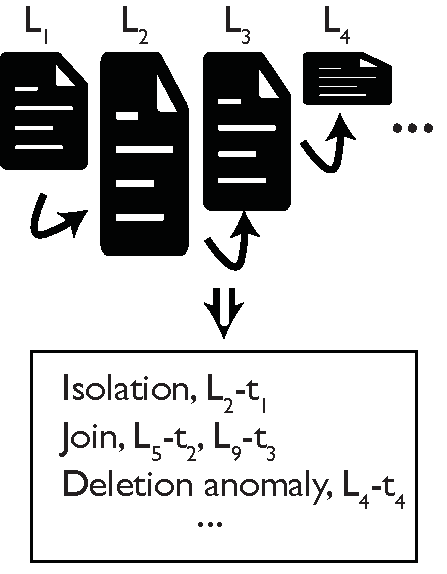
\includegraphics[height=2in]{indexingTask.pdf}
       \caption{\textnormal{The task to be solved by the algorithms
           and human indexers. Construct an index into ordered video
           lecture transcripts such that index keywords and phrases
           reference the lecture portions where corresponding concepts
           are introduced.}}
       \label{fig:task}
\end{figure}

The ordered lecture transcripts $L_1$--$L_n$ contain lines of
instructor speech, together with timing information. An index is to be
constructed that maps concept-bearing words and phrases to
lecture-time pairs. Note that index entries may map to multiple
lectures, if the corresponding word or phrase is important in those
lectures. Our current implementations set $t_n$ to the first
occurrence of the respective index term in the lecture.
Note as well that we do not impose a controlled vocabulary for the
index entries. All entries are taken from the transcript text. Any
word or phrase is therefore a potential candidate for inclusion in the
index. 

Our first experiment took a traditional approach, selecting words for
the index that appeared disproportionately often in certain
lectures. We then incorporated lexical information, by only
considering phrases that followed certain part-of-speech
patterns. Finally, we introduced external knowledge from Wikipedia
into an algorithm's indexing decisions. Note that none of the
algorithms included supervised learning, as we do not assume the
existence of a training set for all courses.

In Section~\ref{sec:relWork} we review some of the related
literature. Section~\ref{sec:gold} offers more detail on how we
created our three human-generated reference
indexes. Section~\ref{sec:exp} introduces the algorithms we
explored. Section~\ref{sec:discussion} offers some observations around
the experimental results, and we conclude in a final section.


%% This task of forming an index over the lectures in an online course,
%% which we refer to as the keyword extraction task, is inherently
%% difficult. A human performing the task must have a deep understanding
%% of the concepts in each lecture, as well as their role in the broader
%% context of the entire course. A 25 minute lecture video might have
%% around 4500 individual words, from which the algorithm must form
%% around 20 phrases to capture the content of the lecture. There is a
%% certain amount of subjectivity inherent in the task, and there can be
%% differing reasonable interpretations of what should be considered a
%% keyword. When humans select important phrases from a lecture they use
%% previous knowledge - for example, in a databases course one might use
%% previous knowledge of functional dependencies to decide that
%% ``Armstrong's Axiom'' should be one of the keyphrases - and we draw on
%% this strategy to automatically decide on keyphrases.


